%! suppress = LineBreak
%! suppress = MissingLabel

Как мы убедились ранее (см.~\ref{subsec:all-interpreters}), программирование состоит из написания новых и новых интерпретаторов поверх друг друга.
Интерпретаторы задают семантику новых языков (см~\ref{subsubsec:semantics}).
В классическом виде язык задаётся как множество деревьев, а интерпретатор отправляет деревья в объект мета-языка.
Если язык встроенный, то такой подход называют deep embedding (см.~\ref{subsubsec:edsl}).
\[
    \sembr{\bullet} : L \to D
\]

Можно заметить, что в конечном итоге мы используем только элемент домена, в который интерпретатор отображает программу.
Сама программа же представляет собой лишь удобную синтаксическую запись элемента домена и является промежуточным шагом, а не самоцелью.
В то же время доменом в случае встроенных языков, заданных интерпретаторами, являются объекты мета-языка.
Можем ли мы миновать стадию интерпретации собственного синтаксиса и сразу строить объект домена в синтаксисе мета-языка?
Да, такое встраивание называется shallow embedding, о нём эта глава.

\subsection{Формальный путь в зазеркалье}

\subsubsection{Рекурсивные структуры через функторы}

Любой рекурсивный тип данных можно представить с помощью двух типов: один отвечает за форму структуры, второй --- за рекурсивность.
Рассмотрим для примера дерево.
\begin{minted}{haskell}
    data Tree a = Leaf a | Node a (Tree a) (Tree a)
\end{minted}

Строим тип, отвечающий за форму, параметризуясь по дополнительному типовому параметру и заменяя все рекурсивные ссылки на него.
Идея аналогична написанию рекурсивных функций через комбинатор неподвижной точки.
\begin{minted}{haskell}
    data Shape a rec = Leaf a | Node a rec rec
\end{minted}

За рекурсивность будет отвечать комбинатор неподвижной точки уровня типов.
Он передаёт последним типовым параметром в форму рекурсивный тип.
\begin{minted}{haskell}
    data Fix shape = In { out :: shape (Fix shape) }
\end{minted}

Можно показать, что старое и новое представление деревьев изоморфны, следовательно, взаимозаменимы: \mintinline{haskell}|Tree a ?$\simeq$? Fix (Shape a)|.

\begin{task}
    Какие типы будут у \mintinline{haskell}|In| и \mintinline{haskell}|out|?
\end{task}

\begin{task}
    Покажите, что \mintinline{haskell}|Tree a ?$\simeq$? Fix (Shape a)|.
\end{task}

Типы форм объявляют функторами, чтобы иметь возможность подменять рекурсивные ссылки чем-то другим и наоборот (примеры увидим далее):
\begin{minted}{haskell}
    instance Functor (Shape a) where
      fmap :: (b -> c) -> Shape a b -> Shape b c
      fmap f = \case Leaf x -> Leaf x; Node x l r -> Node x (f l) (f r)
\end{minted}

\subsubsection{Категории и алгебры}

Посмотрим совсем немного теории категорий.

\vocab{Категория} --- это коллекция объектов и коллекция стрелок.
Для каждого объекта $X$ существует тождественная стрелка, а для каждой пары стрелок существует способ получить их композицию: $f : Y \to Z, g : X \to Y \Rightarrow f \circ g : X \to Z$.

Определяют категорию, соответствующую Haskell --- $Hask$.
На самом деле это плохая категория с точки зрения теории, но для наших нестрогих рассуждений подойдёт\footnote{\url{https://math.andrej.com/2016/08/06/hask-is-not-a-category/}}.
Объектами в Hask являются типы языка Haskell, а морфизмами --- термы, задающие функции между соответствующими типами.
Тождественный морфизм --- \mintinline{haskell}|id|, композиция задаётся как \mintinline{haskell}|f . g = \x -> f (g x)|.

\begin{task}
    Как в такой категории представить константы?
\end{task}

\vocab{Функтором} называется отображение между категориями, которое объектам одной категории сопоставляет объекты другой, а стрелкам одной --- стрелки другой.
В Haskell типовые конструкторы задают отображение между объектами, а \mintinline{haskell}|fmap| --- между стрелками.
Функтор должен сохранять тождественный морфизм и композицию.
\begin{figure}[h!]
    \centering
    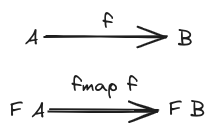
\includegraphics[width=0.25\textwidth]{figs/functor}
\end{figure}

\vocab{Алгеброй} в категории $C$ называется пара из объекта категории $X \in Obj(C)$ и морфизма $\phi : F\ap X \to X$, где $F$ --- функтор.
Сам морфизм $F\ap X \to X$ называют \vocab{f-алгеброй}.
Алгебрами в смысле категорий можно описывать алгебры.
Так, в качестве объекта $X$ берём носитель алгебры.
В качестве функтора $F$ --- сигнатуру алгебры в виде типа-формы.
Тогда морфизмом будет интерпретация сигнатуры.
\begin{minted}{haskell}
    data MonoidSig carrier = Mempty | Mappend carrier carrier

    interpretSig :: MonoidSig Int -> Int
    interpretSig = \case Mempty -> 0; Mappend l r -> l + r
\end{minted}

\begin{task}
    Реализуйте алгебру печати, какой тип должен выступить носителем?
\end{task}

\vocab{Морфизмом алгебр} называется такой морфизм между носителями $h : X \to Y$, что следующая диаграмма коммутирует.
Говорят, что \vocab{диаграмма коммутирует}, если все возможные пути по стрелкам в ней равны.
\begin{figure}[h!]
    \centering
    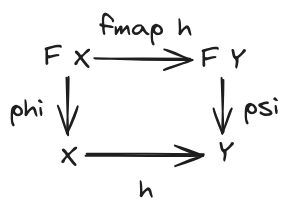
\includegraphics[width=0.3\textwidth]{figs/alg-homomorphism}
\end{figure}

В морфизме алгебр можно обнаружить знакомые черты гомоморфизмов, то есть операций между носителями, которые ``уважают'' операции сигнатуры алгебраической теории.

Алгебры над категорией $C$ образуют \vocab{категорию алгебр}, в которой объектами являются алгебры, а морфизмами --- морфизмы алгебр.

\subsubsection{Рекурсивные типы в категориях}

\vocab{Начальным (инициальным) объектом} категории называется объект, из которого в каждый другой объект существует уникальная стрелка.
\vocab{Терминальным (финальным) объектом} категории называется объект, в который из каждого другого объекта категории существует уникальная стрелка.

Инициальный и терминальный объекты категории не обязательно присутствуют в единственном экземпляре.
Но все инициальные объекты изоморфны друг другу, как и все терминальные.

\begin{task}
    Приведите начальный и терминальный объекты категории $Hask$.
\end{task}

Рекурсивный тип --- это тип, значит ему соответствует объект в категории Hask.
$X$ является рекурсивным типом с формой $F$, если имеет место следующий изоморфизм:
\[X \simeq F\ap X\]

Можно заметить, что свидетель изоморфизма справа налево напоминает f-алгебру, а слева направо --- f-коалгебру (всё то же самое, только все стрелки в обратную сторону).
И действительно, подходящий объект $X$ должен быть либо начальным объектом категории алгебр, либо терминальным объектом категории коалгебр (с соответствующими морфизмами).
Первый вариант соответствует конечным структурам данных, второй --- потенциально бесконечным.

Начальным объектом категории алгебр над $Hask$ для функтора $f$ является следующая алгебра: \mintinline{haskell}|(Fix f, In)| (покажем это далее).
Более того, терминальным объектом категории коалгебр будет \mintinline{haskell}|(Fix f, out)|, благодаря ленивости Haskell.

% todo

\subsubsection{Катаморфизмы: туда и обратно}

Покажем, что \mintinline{haskell}|(Fix f, In)| является инициальным\footnote{\url{https://bartoszmilewski.com/2017/02/28/f-algebras/}}\footnote{\url{https://ncatlab.org/nlab/show/catamorphism}}.
Действительно, для каждого типа \texttt{a} и для каждой f-алгебры \texttt{phi} мы можем построить такой морфизм \mintinline{haskell}|cata phi :: Fix f -> a|, что следующая диаграмма будет коммутировать.
\begin{figure}[h!]
    \centering
    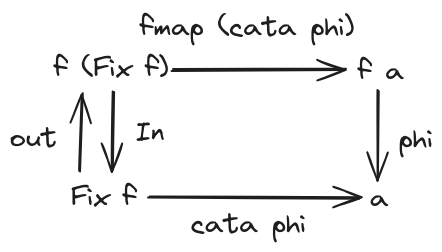
\includegraphics[width=0.4\textwidth]{figs/cata}
\end{figure}

Из диаграммы сразу видно, как такой морфизм построить.
Его называют \vocab{катаморфизмом} f-алгебры \texttt{phi}.
Он является универсальной свёрткой рекурсивных структур данных\footnote{\url{https://reasonablypolymorphic.com/blog/recursion-schemes/index.html}}~\cite{meijer1991functional, meijer1995bananas}, с которой начинается наука рекурсивных схем, ``структурного'' функционального программирования без неструктурной рекурсии.
\begin{minted}{haskell}
    cata :: Functor f => (f a -> a) -> Fix f -> a
    cata phi = phi . fmap (cata phi) . out
\end{minted}

Катаморфизм сначала обрабатывает рекурсивные ссылки, добираясь к ним с помощью \mintinline{haskell}|fmap|, и сворачивает поддеревья, оставляя результаты вместо бывших вхождений поддеревьев.
Таким образом, получается тип формы, у которого вместо рекурсивных ссылок уже значения нужного типа \texttt{a}, а его уже можно непосредственно свернуть с помощью f-алгебры.

% todo картинка из презы

\begin{task}
    Убедитесь, что печатающая алгебра действительно сворачивает терм в строчку.
\end{task}

Покажем, что \mintinline{haskell}|(Fix f, In)| является ещё и терминальным объектом.
Аналогично, для каждого объекта \texttt{a} и f-коалгебры \texttt{psi} найдётся морфизм \mintinline{haskell}|ana psi :: a -> Fix f|.
\begin{figure}[h!]
    \centering
    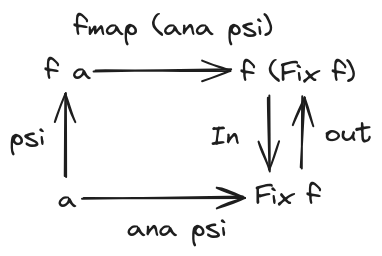
\includegraphics[width=0.35\textwidth]{figs/ana}
\end{figure}

\begin{minted}{haskell}
    ana :: Functor f => (a -> f a) -> a -> Fix f
    ana psi = In . fmap (ana psi) . psi
\end{minted}

Анаморфизм является универсальной развёрткой.
f-коалгебра показывает, как из некоторого значения получить один слой структуры данных (тип-формы).
Он вместо рекурсивных ссылок хранит зёрнышки, из которых потом прорастут поддеревья.
Анаморфизм как раз сначала разворачивает один слой, а потом рекурсивно разворачивает все поддеревья.

Анаморфизм проясняет интуицию, почему терминальными коалгебрами кодируют потенциально бесконечные структуры данных.
f-коалгебра по некоторому зерну вычисляет следующий слой структуры.
Так, можно слой за слоем лениво вычислять поддеревья, потенциально сколь угодно долго.

С помощью катаморфизма можно получить изоморфизм между структурами данных и их свёртками:
\mintinline{haskell}|Fix f ?$\simeq$? forall a . (f a -> a) -> a|.
\begin{minted}{haskell}
    to :: Functor f => Fix f -> (forall a . (f a -> a) -> a)
    to = flip cata

    from :: (forall a . (f a -> a) -> a) -> Fix f
    from g = g Fix
\end{minted}

% todo пример со списком

\subsubsection{Алгебраическое представление типа}

\begin{figure}[h!]
    \centering
    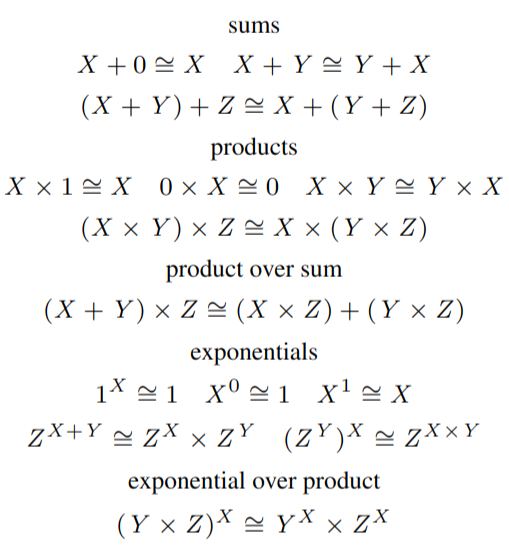
\includegraphics[width=0.4\textwidth]{/home/yukio/Diary/projs/fpcourse/fp-2024/docs/figs/school-alg}
    \caption{Законы школьной алгебры ностальгии ради~\cite{hinze2010reason}.}
    \label{fig:school-alg}
\end{figure}

% todo reason isomorphically
% todo connection with cardinalities

\cite[глава 1]{maguire-types}

% todo каноническое представление типа

% todo

\subsubsection{Прибытие в зазеркалье}

Вспомним, что нашей целью было конструирование программ напрямую как объектов мета-языка (домена).
\[
    \sembr{\bullet} : L \to D
\]

Для этого воспользуемся изоморфизмом
\mintinline{haskell}|Fix f ?$\simeq$? forall d . (f d -> d) -> d|, который говорит о том, что правую часть можно использовать вместо левой.
Иначе говоря, вместо того, чтобы конструировать дерево языка \mintinline{haskell}|Fix f|, достаточно сконструировать функцию мета-языка с типом справа, которая и будет выполнять роль терма нового языка.

Действительно, выбирая тип-домен \texttt{d} и передавая соответствующую алгебру, мы можем получать различные интерпретации термов зазеркалья.

TODO % todo пример

Мы ещё избавились не от всех деревьев в программе --- остался функтор, задающий форму.
Представим его в канонической форме и с помощью алгебраических преобразований получим функцию без единой структуры данных.

TODO % todo преобразования

В качестве примера покажем, что список Чёрча (да и в целом кодирование по Чёрчу) является зазеркальной альтернативой обычного списка\footnote{\url{https://okmij.org/ftp/tagless-final/course/Boehm-Berarducci.html}}.

TODO % todo пример

Если зафиксировать интерпретацию, то функции-аргументы можно реализовать статически и просто ссылаться на них в терме.
Таким образом, про объявление функций можно думать как про расширение некоторого встроенного предметного языка.
Сравните:
\begin{figure}[h]
    \centering
    \begin{tabular}{|p{0.45\linewidth}|p{0.45\linewidth}|}
        \hline
        Deep                                                                                                    & Shallow                                                    \\
        \hline
        Синтаксис языка задаётся набором допустимых нод дерева                                                  & Декларация функции задаёт новую ноду дерева: вызов этой функции       \\
        \hline
        Интерпретатор при виде каждой ноды выполняет соответствующий код на мета-языке (ветку паттерн-матчинга) после вычисления поддеревьев & Интерпретатор при виде вызова выполняет код тела функции после вычисления аргументов
        \hline
    \end{tabular}
\end{figure}

Общие рассуждения про shallow embeddings, свёртки и библиотеки можно почитать в~\cite{gibbons2013functional, gibbons2014folding}.

% todo деревянный язык это бейзлайн

% todo connections to polarity https://ncatlab.org/nlab/show/polarity+in+type+theory

\subsection{Tagless final интерпретаторы}



Это Church encoding с классами типов.


% todo

% todo meta-circular

% todo композиционность и её восстановление через эксплицирование контекстных зывисимостей.

% todo вместо того, чтобы доставлять объект к месту деконструирования, доставляем меcто деконструирования к месту конструирования

% todo bananas in space и что там было про функции и зачем

\subsection{Использование зазеркалья в реальности}

% todo visitor pattern
% todo reactive programming https://youtu.be/sTSQlYX5DU0?si=Ybxux16h5Vt1LnC4

% todo pull and push

\subsubsection{Expression problem}

% todo wadler the expression problem
% todo https://homepages.inf.ed.ac.uk/wadler/papers/expression/expression.txt

% todo Extensibility for the Masses: Practical Extensibility with Object Algebras

% todo

\subsubsection{Deforestation \& fusion}

% todo Reading circle about fusion

% todo haskell inlining
% todo Oleg about fusion and streams
% todo fused effects

% todo short cut to deforestation
% todo stream fusion from lists to streams to nothing at all
% todo call-pattern specialization for Haskell programs

% todo https://markkarpov.com/tutorial/ghc-optimization-and-fusion.html

% todo FRP

% todo visitors

% todo

\subsubsection{Codata}

% todo codata, copattern-matching
% todo are custom patterns in haskell connected to this?

% todo

\subsubsection{Threaded code}

% todo https://en.wikipedia.org/wiki/Threaded_code
